\documentclass[10pt,a4paper]{article}
\usepackage[utf8]{inputenc}
\usepackage[margin=1.3cm,top=1.6cm,bottom=1.6cm]{geometry}
\usepackage{graphicx}
\usepackage{xcolor}
\usepackage{booktabs}
\usepackage{listings}
\usepackage{fancyhdr}
\usepackage{hyperref}
\usepackage{enumitem}

\definecolor{codegreen}{rgb}{0.1,0.55,0.2}
\definecolor{codegray}{rgb}{0.45,0.45,0.45}
\definecolor{codepurple}{rgb}{0.55,0.1,0.65}
\definecolor{backcolour}{rgb}{0.96,0.97,0.98}
\definecolor{bordercolour}{rgb}{0.85,0.88,0.92}
\definecolor{brandblue}{rgb}{0.08,0.28,0.52}

\lstdefinestyle{javastyle}{
    backgroundcolor=\color{backcolour},
    commentstyle=\color{codegreen}\itshape,
    keywordstyle=\color{brandblue}\bfseries,
    numberstyle=\tiny\color{codegray},
    stringstyle=\color{codepurple},
    basicstyle=\ttfamily\scriptsize,
    breakatwhitespace=false,
    breaklines=true,
    captionpos=b,
    keepspaces=true,
    numbers=none,
    showspaces=false,
    showstringspaces=false,
    showtabs=false,
    tabsize=2,
    frame=single,
    rulecolor=\color{bordercolour}
}
\lstset{style=javastyle}

\hypersetup{
    colorlinks=true,
    linkcolor=brandblue,
    urlcolor=brandblue,
    citecolor=brandblue
}

\pagestyle{fancy}
\fancyhf{}
\lhead{\scriptsize\textbf{ShP-2216 Software Design Patterns} \textbar\ Assignment 4: Facade Pattern}
\rhead{\scriptsize\textbf{Astana IT University} \textbar\ SE-2537}
\lfoot{\scriptsize Dias Tursynbay (SE-2537)}
\rfoot{\scriptsize Page \thepage\ of 3}
\renewcommand{\headrulewidth}{0.5pt}
\renewcommand{\footrulewidth}{0.5pt}

\begin{document}

% Title Header
\begin{center}
    {\large\bfseries\color{brandblue} Assignment 4: Facade Pattern Design \& Evaluation}\\[2pt]
    {\small\textbf{Simplifying Complex Media Conversion Subsystems via Higher-Level Orchestration}}
\end{center}
\vspace{-8pt}

\noindent
\begin{tabular*}{\linewidth}{@{\extracolsep{\fill}}p{0.48\linewidth}p{0.48\linewidth}@{}}
\textbf{Student:} Dias Tursynbay (SE-2537) & \textbf{Course:} ShP-2216 Software Design Patterns \\
\textbf{Topic:} Option A (Media/File Conversion Facade) & \textbf{Instructor:} Yerassyl Bekenov (AITU, Year 2, Tri 4) \\
\textbf{Repository:} \url{https://github.com/HumbleCherry10/SDP-4.git} & \textbf{Language \& Runtime:} Java (JDK 17 Adoptium) \\
\textbf{Base Commit:} \texttt{828ea5a} \textbar\ \textbf{Final:} \texttt{1ae59a6} & \textbf{Status:} 4/4 Automated Checks Passed (\textsc{Demo 1--4 PASS})
\end{tabular*}

\vspace{3pt}
\hrule
\vspace{4pt}

\subsection*{1. Subsystem Complexity \& Facade Pattern Rationale}
In real-world multimedia software, converting an audio or video file from one container format to another is an inherently complex operation spanning multiple decoupled subsystem components with strict temporal and operational dependencies:
\begin{enumerate}[noitemsep,topsep=1pt,leftmargin=1.5em]
    \item \textbf{Container Header Parsing:} Inspecting the raw file container to retrieve stream metadata and duration (\texttt{MetadataReader}).
    \item \textbf{Codec Resolution:} Querying a codec registry to instantiate appropriate compression algorithms matching container requirements (\texttt{CodecFactory}, \texttt{MPEG4CompressionCodec}, \texttt{OggCompressionCodec}).
    \item \textbf{Bitstream Reading \& Bitrate Transcoding:} Reading raw byte buffers and resampling bitrates between mismatched codecs (\texttt{BitrateReader}).
    \item \textbf{Audio Post-Processing:} Demuxing audio channels, performing gain normalization, and mastering stereo audio tracks (\texttt{AudioMixer}).
\end{enumerate}

\textbf{Problem Without a Facade:} Direct client interaction with these four subsystems creates severe architectural defects. Client code becomes tightly coupled to low-level byte arrays, must duplicate instantiation order across every conversion call, and is vulnerable to breaking whenever internal subsystem APIs evolve.

\textbf{Solution via Facade:} The \texttt{MediaConversionFacade} introduces a clean, higher-level abstraction. It exposes a single self-explanatory method \texttt{convertMedia(String fileName, String targetFormat)}. The Facade encapsulates the multi-step orchestration pipeline. Crucially, the subsystem classes remain \textbf{unaware of the Facade} (zero back-references). Power users and advanced clients can still bypass the Facade and use subsystem classes directly, preserving full flexibility.

\subsection*{2. Complete UML Class Diagram \& Architectural Role Mapping}
\begin{center}
    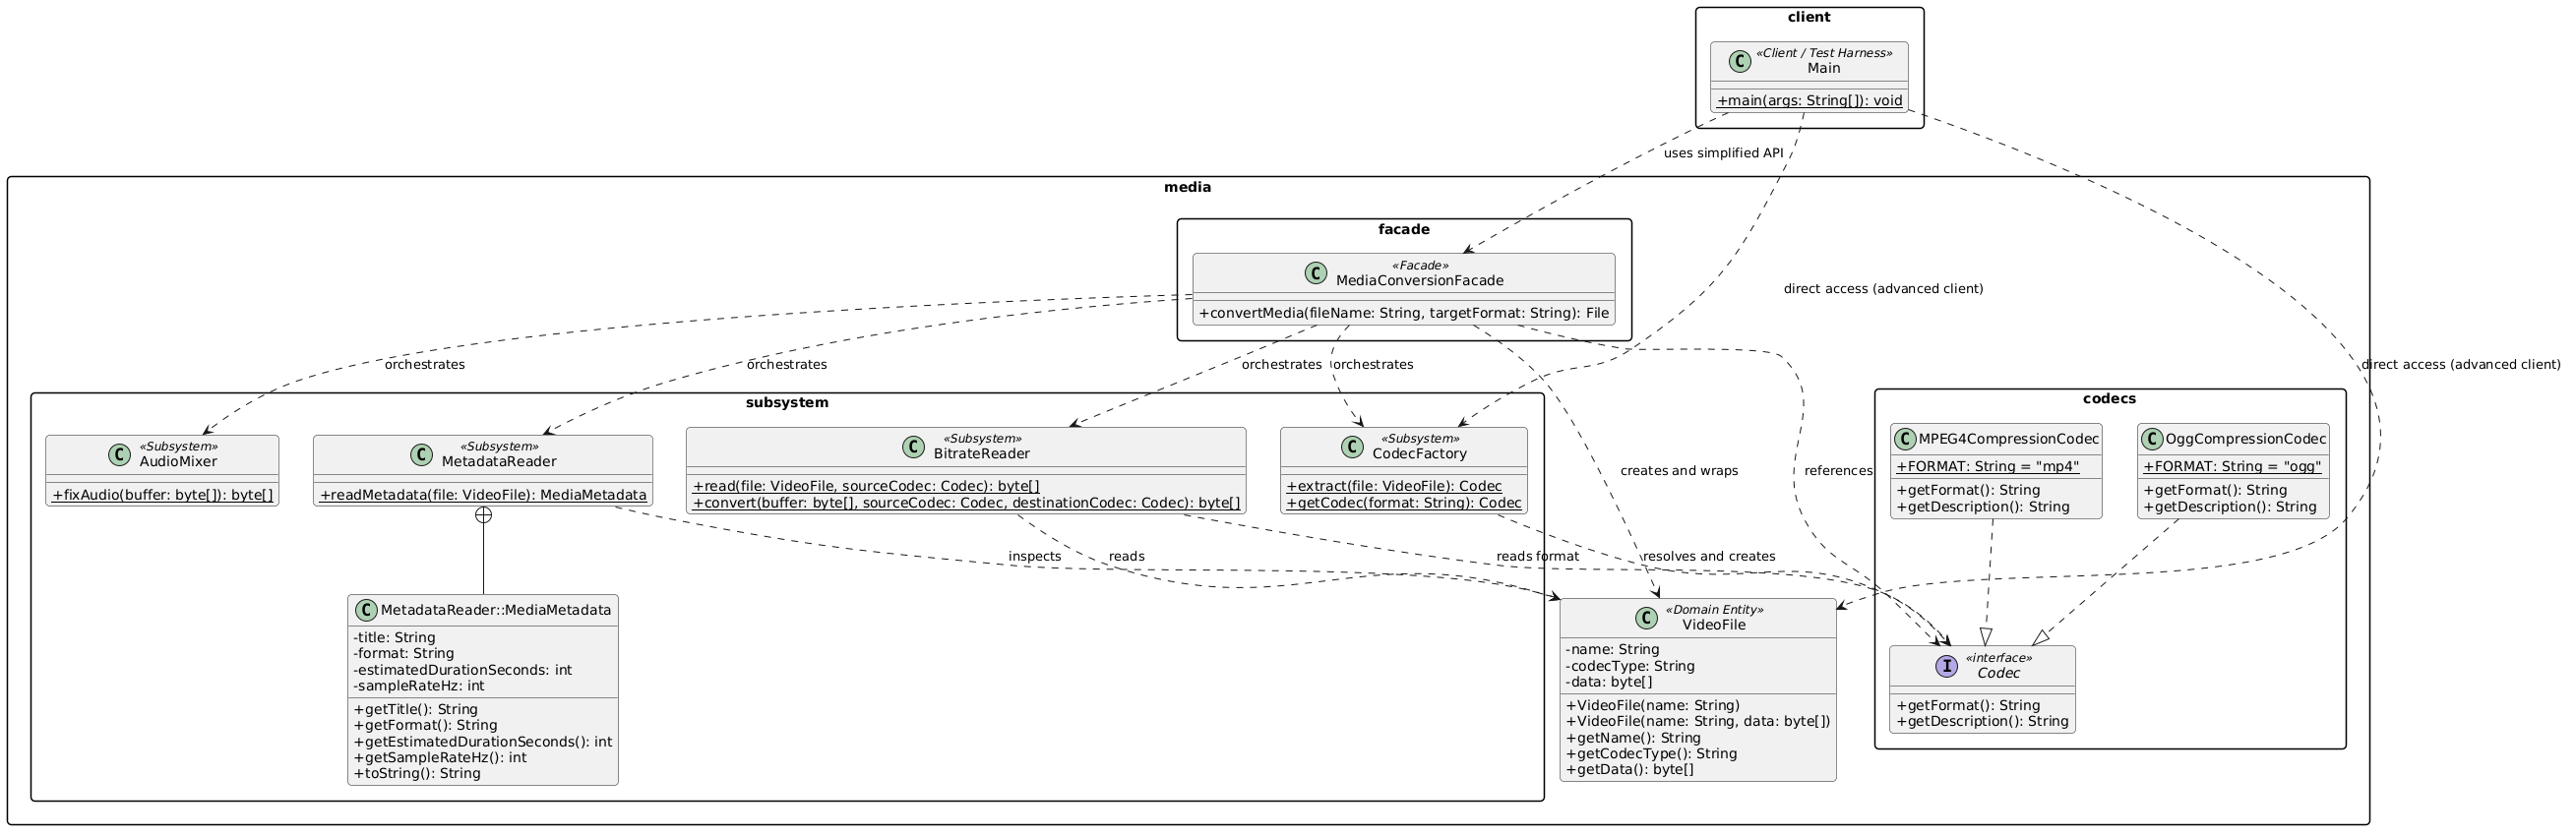
\includegraphics[width=0.74\linewidth]{uml_diagram.png}\\[1pt]
    \scriptsize \textbf{Figure 1:} Complete UML Class Diagram showing Client, Facade, Codecs, and Subsystem Classes.
\end{center}

\vspace{-6pt}
\noindent
\begin{tabular*}{\linewidth}{@{\extracolsep{\fill}}p{0.18\linewidth}p{0.25\linewidth}p{0.18\linewidth}p{0.32\linewidth}@{}}
\toprule
\textbf{Role} & \textbf{Class Name} & \textbf{Package} & \textbf{Core Responsibility} \\
\midrule
\textbf{Facade} & \texttt{MediaConversionFacade} & \texttt{media.facade} & Coordinates conversion pipeline behind \texttt{convertMedia()}. \\
\textbf{Subsystem 1} & \texttt{MetadataReader} & \texttt{media.subsystem} & Parses file headers and returns container stream metadata. \\
\textbf{Subsystem 2} & \texttt{CodecFactory} & \texttt{media.subsystem} & Extracts source codec and instantiates destination codecs. \\
\textbf{Codec Interface} & \texttt{Codec} (Interface) & \texttt{media.codecs} & Contract for concrete compression codecs (\texttt{mp4}, \texttt{ogg}). \\
\textbf{Subsystem 3} & \texttt{BitrateReader} & \texttt{media.subsystem} & Reads media bitstream and transcodes buffer between codecs. \\
\textbf{Subsystem 4} & \texttt{AudioMixer} & \texttt{media.subsystem} & Equalizes audio channels and normalizes multi-track audio. \\
\textbf{Domain Model} & \texttt{VideoFile} & \texttt{media} & Encapsulates filename, format extension, and simulated payload. \\
\textbf{Client / Harness} & \texttt{Main} & \texttt{client} & Tests facade conversions, error handling, and direct subsystem access. \\
\bottomrule
\end{tabular*}

\clearpage

\subsection*{3. Clean Code Implementation Analysis (Five Annotated Excerpts)}
The project adheres strictly to Clean Code standards (Robert C. Martin). Below are five concrete excerpts illustrating separated responsibilities, meaningful names, encapsulation, small cohesive classes, and defensive error handling.

\subsubsection*{Excerpt 1: Meaningful, Intention-Revealing Method Names (\texttt{Main.java})}
\textbf{Principle:} \textit{Meaningful Names (Clean Code Ch. 2) \& Intent-Revealing Interfaces}
\begin{lstlisting}[language=Java]
// Client interacts with an intuitive, domain-level verb:
File mp4Result = facade.convertMedia("summer_trip.ogg", "mp4");
\end{lstlisting}
\textbf{Design Benefit:} Instead of forcing the client to decipher low-level subsystem primitives like \texttt{BitrateReader.convert(read(...))}, the Facade provides a self-documenting method name \texttt{convertMedia}. The intent is immediately transparent without requiring secondary documentation.

\subsubsection*{Excerpt 2: Pure Orchestration Without Reimplementation (\texttt{MediaConversionFacade.java})}
\textbf{Principle:} \textit{Single Responsibility Principle (SOLID - SRP)}
\begin{lstlisting}[language=Java]
// Facade orchestrates steps in order without implementing codec or mixing algorithms:
VideoFile file = new VideoFile(fileName);
MetadataReader.MediaMetadata metadata = MetadataReader.readMetadata(file);
Codec sourceCodec = CodecFactory.extract(file);
Codec destinationCodec = CodecFactory.getCodec(targetFormat);
byte[] rawBuffer = BitrateReader.read(file, sourceCodec);
byte[] convertedBuffer = BitrateReader.convert(rawBuffer, sourceCodec, destinationCodec);
byte[] finalBuffer = AudioMixer.fixAudio(convertedBuffer);
\end{lstlisting}
\textbf{Design Benefit:} The Facade has one reason to change: modifications to the high-level conversion workflow. It delegates codec decoding to \texttt{CodecFactory}, bitrate resampling to \texttt{BitrateReader}, and audio mixing to \texttt{AudioMixer}, completely avoiding bloated ``God Object'' anti-patterns.

\subsubsection*{Excerpt 3: Information Hiding \& Zero Subsystem Leakage (\texttt{MediaConversionFacade.java})}
\textbf{Principle:} \textit{Encapsulation \& Law of Demeter}
\begin{lstlisting}[language=Java]
public File convertMedia(String fileName, String targetFormat) { ... }
\end{lstlisting}
\textbf{Design Benefit:} No internal subsystem types (\texttt{Codec}, \texttt{MediaMetadata}, \texttt{byte[]}, \texttt{BitrateReader}) leak through the public interface. The caller provides standard primitives (\texttt{String}) and receives a high-level file descriptor (\texttt{java.io.File}). Subsystem refactoring can occur with zero impact on calling clients.

\subsubsection*{Excerpt 4: Small, Focused Classes with High Cohesion (\texttt{AudioMixer.java})}
\textbf{Principle:} \textit{Small, Single-Purpose Classes (Clean Code Ch. 3)}
\begin{lstlisting}[language=Java]
public class AudioMixer {
    public static byte[] fixAudio(byte[] buffer) {
        if (buffer == null) throw new IllegalArgumentException("Audio buffer must not be null.");
        System.out.println("[AudioMixer] Normalizing audio channels, applying gain staging, and mixing...");
        String content = new String(buffer, StandardCharsets.UTF_8);
        return (content + " + [AudioMixer: Normalized 48kHz Stereo Master]").getBytes(StandardCharsets.UTF_8);
    }
}
\end{lstlisting}
\textbf{Design Benefit:} \texttt{AudioMixer} is constrained strictly to audio channel processing. It does not inspect video frames, manage file handles, or resolve codecs. High cohesion ensures that audio processing logic is testable and maintainable in isolation.

\subsubsection*{Excerpt 5: Defensive Validation \& Graceful Error Handling (\texttt{CodecFactory.java})}
\textbf{Principle:} \textit{Robust Error Handling \& Fail-Fast Guards (Clean Code Ch. 7)}
\begin{lstlisting}[language=Java]
public static Codec getCodec(String format) {
    if (format == null || format.trim().isEmpty()) {
        throw new IllegalArgumentException("Format specification must not be null or empty.");
    }
    String normalized = format.trim().toLowerCase();
    if (normalized.startsWith(".")) normalized = normalized.substring(1);
    switch (normalized) {
        case "mp4": return new MPEG4CompressionCodec();
        case "ogg": return new OggCompressionCodec();
        default:    throw new UnsupportedOperationException("Codec not supported for format: ." + format);
    }
}
\end{lstlisting}
\textbf{Design Benefit:} Inputs are validated immediately before execution. Unsupported formats fail fast with explicit exceptions (\texttt{UnsupportedOperationException}) instead of allowing corrupted streams or obscure \texttt{NullPointerException} failures downstream.

\clearpage

\subsection*{4. Conclusion: What the Facade Hides vs. What Remains Accessible}

\subsubsection*{What the Facade Hides (Encapsulated Complexity)}
\begin{itemize}[noitemsep,topsep=1pt,leftmargin=1.5em]
    \item \textbf{Component Instantiation \& Dependency Lifecycle:} The client is relieved from instantiating 4 separate subsystem classes and passing objects between them.
    \item \textbf{Strict Execution Sequencing:} The internal sequence (Parse Metadata $\to$ Detect Source Codec $\to$ Resolve Target Codec $\to$ Read Bitstream $\to$ Transcode $\to$ Normalize Audio) is enforced by the Facade, eliminating order-of-operation defects.
    \item \textbf{Low-Level Buffer Management:} Intermediate byte arrays and bitrate adjustments remain strictly internal.
\end{itemize}

\subsubsection*{What Remains Directly Accessible (Decoupled Flexibility)}
\begin{itemize}[noitemsep,topsep=1pt,leftmargin=1.5em]
    \item \textbf{Zero Back-References:} Subsystem classes (\texttt{MetadataReader}, \texttt{CodecFactory}, \texttt{BitrateReader}, \texttt{AudioMixer}) contain no references or imports to \texttt{MediaConversionFacade}.
    \item \textbf{Direct Usability for Advanced Clients:} As proven in \textbf{DEMO 4}, advanced clients can instantiate subsystem components directly to perform custom pipelines (e.g., custom bitrates, alternative audio mixes, or direct buffer manipulation) without restriction.
\end{itemize}

\subsubsection*{Architectural Trade-Off Analysis}
\noindent
\begin{tabular*}{\linewidth}{@{\extracolsep{\fill}}p{0.48\linewidth}p{0.48\linewidth}@{}}
\toprule
\textbf{Advantages of Facade} & \textbf{Architectural Trade-offs / Limitations} \\
\midrule
$\bullet$ Reduces client cognitive load to a single call. & $\bullet$ May become a ``God Object'' if new features are added without care. \\
$\bullet$ Eliminates tight coupling between client and subsystems. & $\bullet$ High-level API may not expose fine-grained flags needed by experts. \\
$\bullet$ Centralizes workflow and error-handling logic. & $\bullet$ Introduces an additional layer of method indirection. \\
\bottomrule
\end{tabular*}

\subsection*{5. Automated Demonstration Checks \& Output Verification}
The test suite in \texttt{Main.java} executes four deterministic checks covering standard facade use, format reversal, error handling, and direct subsystem access. All four checks execute and pass:
\begin{itemize}[noitemsep,topsep=1pt,leftmargin=1.5em]
    \item \textbf{DEMO 1 (PASS):} Standard OGG $\to$ MP4 conversion via Facade (\texttt{summer\_trip\_converted.mp4}).
    \item \textbf{DEMO 2 (PASS):} Reverse MP4 $\to$ OGG conversion via Facade (\texttt{presentation\_converted.ogg}).
    \item \textbf{DEMO 3 (PASS):} Gracefully catches \texttt{UnsupportedOperationException} when requesting unsupported format \texttt{.avi}.
    \item \textbf{DEMO 4 (PASS):} Advanced client executes custom pipeline bypassing Facade (\texttt{raw\_footage\_custom.mp4}).
\end{itemize}

\subsection*{6. Defense Guide \& Rapid Oral Walkthrough}
\begin{itemize}[noitemsep,topsep=1pt,leftmargin=1.5em]
    \item \textbf{1. Live Demonstration:} Execute \texttt{java -cp out Main}. Point out that standard conversions happen in 1 line of code, exceptions are gracefully caught, and DEMO 4 proves direct subsystem usability with \textbf{4/4 CHECKS PASSED}.
    \item \textbf{2. What does Facade hide and why? (CLO 3):} Point to \texttt{convertMedia()}. Explain that it hides the 6-step coordination sequence, codec resolution, and byte buffer transformations so the client has zero coupling to subsystem internals.
    \item \textbf{3. Why are subsystem classes unaware of the Facade? (CLO 1 \& 2):} Show that \texttt{AudioMixer.java} and \texttt{CodecFactory.java} have zero imports of \texttt{MediaConversionFacade}. Emphasize that the Facade is a unidirectional gateway, not an enclosing sandbox.
\end{itemize}

\subsection*{7. Academic References}
\begin{enumerate}[noitemsep,topsep=1pt,leftmargin=1.5em]
    \item Gamma, E., Helm, R., Johnson, R., \& Vlissides, J. (1994). \textit{Design Patterns: Elements of Reusable Object-Oriented Software}. Addison-Wesley.
    \item Martin, R. C. (2008). \textit{Clean Code: A Handbook of Agile Software Craftsmanship}. Prentice Hall.
    \item Freeman, E., \& Robson, E. (2020). \textit{Head First Design Patterns: Facade Pattern}. O'Reilly Media.
    \item Bekenov, Y. (2026). \textit{Lecture 6: Facade Structural Pattern}. Astana IT University, Course ShP-2216.
    \item Refactoring Guru (2026). \textit{Facade Design Pattern in Java}. \url{https://refactoring.guru/design-patterns/facade}.
\end{enumerate}

\end{document}
